% lint-skip: 未完成ステータス（figure/table caption 未対応，人手チェック時に解消予定）
\documentclass[../../main.tex]{subfiles}
\begin{document}

\begin{flushright}
  \footnotesize\textit{【自動文字起こし・要確認】}
\end{flushright}

\noindent
{\bf [解答]} $\triangle O P_n P_{n+1}$ と $\triangle O P_{n+1} P_{n+2}$ の相似比は，
\[
  \dfrac{|O P_{n+1}|}{|O P_n|} \text{ である．} \quad \dots \text{①}
\]
ここで $\triangle O P_0 P_1$ に正弦定理を用いて，
\[
  \dfrac{|O P_1|}{\sin \theta} = \dfrac{\alpha}{\sin(\alpha+\theta)} \implies |O P_1| = \dfrac{\sin \theta}{\sin(\alpha+\theta)} \cdot \alpha \quad \dots \text{②}
\]
だから，$\alpha \neq 0$ より，①から
\[
  \dfrac{|O P_1|}{|O P_0|} = 1 \cdot \dfrac{\sin \theta}{\sin(\alpha+\theta)}
\]
したがって，$0 < \dfrac{\sin \theta}{\sin(\alpha+\theta)} < 1$ ならば $P_n$ は $O$ に収束する． （以上 (イ)）

\begin{figure}[htb]
  \centering
  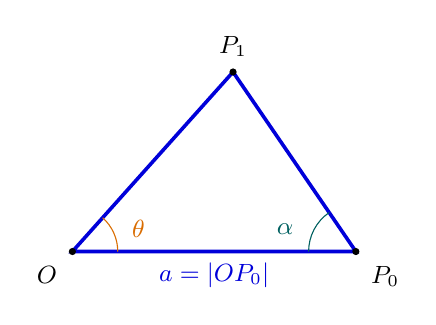
\begin{tikzpicture}[x=1.2cm, y=1.2cm, every node/.style={font=\small}]
    % The sketch follows the problem: theta is at O and alpha at P_0.
    \coordinate (O) at (0,0);
    \coordinate (P0) at (3,0);
    \coordinate (P1) at (1.7,1.9);
    \draw[line width=1.3pt, blue!85!black] (O)--(P0)--(P1)--cycle;
    \draw[thin, orange!85!black] (0.48,0)
    arc[start angle=0, end angle=48.2, radius=0.48];
    \draw[thin, teal!75!black] (2.5,0)
    arc[start angle=180, end angle=124.4, radius=0.5];
    \fill (O) circle(1.3pt) node[below left=2pt] {$O$};
    \fill (P0) circle(1.3pt) node[below right=2pt] {$P_0$};
    \fill (P1) circle(1.3pt) node[above=2pt] {$P_1$};
    \node[orange!85!black] at (0.7,0.24) {$\theta$};
    \node[teal!75!black] at (2.25,0.24) {$\alpha$};
    \node[blue!85!black] at (1.5,-0.25) {$a=|OP_0|$};
  \end{tikzpicture}
  \caption{初項の三角形 $OP_0P_1$ と角 $\theta$，$\alpha$}
  \label{fig:1963_5_initial_triangle}
\end{figure}

\noindent
さて，$\triangle O P_n P_{n+1}$ の面積 $S_n$ とする．まず，
\[
  S_0 = \dfrac{1}{2} |O P_0| |O P_1| = \dfrac{1}{2} \cdot \dfrac{\sin \theta}{\sin(\alpha+\theta)} \alpha^2 \quad \dots \text{③}
\]
であり，①から，$p = \dfrac{\sin \theta}{\sin(\alpha+\theta)}$ として
\[
  S_{n+1} = p^2 S_n
\]
くり返し用いて，③から
\[
  S_n = (p^2)^{n-1} \cdot \dfrac{1}{2} p \alpha^2 = \dfrac{1}{2} p^{2n-1} \alpha^2
\]
したがって，$0 < p < 1$ とあわせて，
\[
  S = \lim_{n \to \infty} \sum_{k=0}^n S_k = \dfrac{1}{2} p \alpha^2 \dfrac{1}{1-p^2}
\]
だから，$S$ は $\triangle O P_0 P_1$ の
\[
  \dfrac{1}{1-p^2} = \dfrac{1}{1 - \left( \dfrac{\sin \theta}{\sin(\alpha+\theta)} \right)^2} \text{ (倍)}
\]
である．(以上 (ロ))

\vspace{0.5cm}

\noindent
ここで，$a_n = |P_n P_{n+1}|$ とおく．①から
\[
  a_{n+1} = p a_n \quad \dots \text{④}
\]
であり，$\triangle O P_0 P_1$ に正弦定理を用いて，
\[
  \dfrac{|P_0 P_1|}{\sin \theta} = \dfrac{\alpha}{\sin(\alpha+\theta)} \implies a_0 = \dfrac{\sin \theta}{\sin(\alpha+\theta)} \alpha
\]
だから，④をくり返し用いて，
\[
  a_n = \dfrac{\sin \theta}{\sin(\alpha+\theta)} \alpha \cdot p^{n-1}
\]
となるので，
\begin{align}
  L &= \lim_{n \to \infty} \sum_{k=0}^n a_k = \dfrac{\sin \theta \cdot \alpha}{\sin(\alpha+\theta)} \cdot \dfrac{1}{1-p} \quad (\because |p| < 1) \\
  &= \dfrac{\sin \theta \cdot \alpha}{\sin(\alpha+\theta)} \cdot \dfrac{\sin(\alpha+\theta)}{\sin(\alpha+\theta) - \sin \theta} = \dfrac{\sin \theta}{\sin(\alpha+\theta) - \sin \theta} \cdot \alpha
\end{align}
である．$\theta \to +0$ として，
\[
  L = \dfrac{\theta}{\sin(\alpha+\theta) - \sin \theta} \cdot \dfrac{\sin \theta}{\theta} \cdot \alpha \longrightarrow \dfrac{\alpha}{\cos \alpha}
\]

\newpage

\end{document}
